\documentclass[12pt,PhD,twoside]{muthesis}
% The regulations say that 12pt should be used
% Change the MSc option to MPhil, MRes or PhD if appropriate

\usepackage{verbatim}
\usepackage{graphicx}
\usepackage{url} % typeset URL's reasonably
\usepackage{listings}

\usepackage{pslatex} % Use Postscript fonts

\usepackage{subcaption}
\usepackage{color}
\usepackage{multirow}
\usepackage{makecell}

\usepackage{mathptmx}
\usepackage{amsmath}

%define some own functions
\newcommand{\tabincell}[2]{\begin{tabular}{@{}#1@{}}#2\end{tabular}} 
\def\D{\mathrm{d}}
% Uncomment the next line if you want subsubsections to be numbered
%\setcounter{secnumdepth}{3}
% Uncomment the next line if you want subsubsections to be appear in
% the table of contents
%\setcounter{tocdepth}{3}

% Uncomment the following lines if you want to include the date as a
% header in draft versions
%\usepackage{fancyhdr}
%\pagestyle{fancy}
%\lhead{}  % left head
%\chead{Draft: \today} % centre head
%\lfoot{}
%\cfoot{\thepage}
%\rfoot{}

\begin{document}
% Uncomment the following lines to leave out list of figures, tables
% and copyright until final printing
%\figurespagefalse
%\tablespagefalse
%\copyrightfalse

\title{Vision/Gesture Recognition using Spiking Neurons}
\author{Qian Liu}

\beforeabstract

\prefacesection{Abstract}
%\abstracttitle
% Single spacing can be turned on for the abstract
%

%The extraction of the report not the research.
%
%The aim, objectives and motivations are... 
%
%What have been done...
%
%The results of experiment...
%
%One sentence about the conclusions and future plan.
%About half page long.

%To explore how the brain may recognise objects in its general,accurate and energy-efficient manner, this paper proposes the use of a neuromorphic hardware system formed from a Dynamic Video Sensor~(DVS)
%silicon retina in concert with the SpiNNaker real-time Spiking Neural
%Network~(SNN) simulator.
%As a first step in the exploration on this platform a recognition system for dynamic hand postures is developed, enabling the study of the methods used in the visual pathways of the brain.
%Inspired by the behaviours of the primary visual cortex, Convolutional Neural Networks (CNNs) are modelled using both linear perceptrons and spiking Leaky Integrate-and-Fire (LIF) neurons.
%
%In this study's largest configuration using these approaches, a network of 74,210 neurons and 15,216,512 synapses is created and operated in real-time using 290 SpiNNaker processor cores in parallel and with 93.0\% accuracy.
%A smaller network using only 1/10th of the resources is also created,
%again operating in real-time, and it is able to recognise the postures
%with an accuracy of around 86.4\% - only 6.6\% lower than the much larger system.
%The recognition rate of the smaller network developed on this neuromorphic system is sufficient for a successful hand posture recognition system, and demonstrates a much improved cost to performance trade-off in its approach.

The human brain recognises huge amount of objects rapidly with ease even in cluttered and natural scenes.
This robust object recognition of the biological system is invariant to the change of position, scale, viewing angle and etc. (known as transformation invariance).
While the major stumbling problem of the computer object recognition lies in the poor robustness to the transformations.

Exploring and mimicking invariant object recognition within the brain is a promising approach to tackling the computational difficulty;
in turn it also contributes to the understanding biological visual processing by means of mimicking neural activity in the visual system of the brain.

Thanks to its high-performance massively parallel processing, SpiNNaker makes it possible to simulate large-scale neural networks in real-time.
Thus, in order to explore the ventral visual pathway of primate brain, this work hires a neuromorphic hardware system formed from a Dynamic Video Sensor~(DVS) silicon retina in concert with SpiNNaker.
As a first step in the exploration, a recognition system for dynamic hand postures is developed on the platform.
Inspired by the behaviours of the primary visual cortex, Convolutional Neural Networks (CNNs) are modelled using both linear perceptrons and Leaky Integrate-and-Fire (LIF) neurons.

Future work is proposed to build an object recognition system with position, scale and view invariance by modelling the hierarchical visual pathway up to the inferotemporal (IT) cortex.
The proposed plan of the system will be able to recognise 200 objects in real time exploiting LIF neurons.



%\afterabstract



% These include the actual text

\chapter{Introduction}
\label{cha:intro}
Patterns or objects in two-dimensional images can be described with four properties~\cite{wysoski2008fast}: position, geometry (i.e. size, area and shape), colour/texture, and trajectory. 
Appearance-based methods are the most direct approach to performing pattern recognition where the test image is compared with a set of templates to find the best match for an individual or combination of properties. 
%In terms of classification algorithms, distance measure methods (nearest neighbour, k-means clustering), support vector machine (SVM), multi-layer perceptron (MLP) neural networks and statistical methods, e.g. Gaussian mixture model (GMM) have been applied successfully in visual recognition. 
However, the 2D projection of an object changes under different conditions including illumination, viewing angles, relative positions and distance, making it virtually impossible to represent all appearances of an object. 
To improve reliability, robustness and classification efficiency, approaches such as edge matching~\cite{canny1986computational}, divide-and-conquer~\cite{toygar2004multiple}, gradient matching~\cite{wei2006robust} and feature based methods~\cite{lowe2004distinctive, bay2008speeded} are used.
%Moreover, feature based methods are used to improve reliability, robustness and classification efficiency. 
%Among various feature extraction methods, the scale-invariant feature transform (SIFT)~\cite{lowe2004distinctive} and the sped-up robust features (SURF)~\cite{bay2008speeded} methods are well-accepted recently in the field. 
Finding a proper feature for a specific object still remains an open question and there is no process as general, accurate, or energy-efficient as that provided by the brain.
It is not a new idea to turn to nature for inspiration. 
%Turning to biology for answers is always the way to explore the field of visual pattern recognition. 
Riesenhuber et al.~\cite{riesenhuber1999hierarchical}, for instance, presented a biologically-inspired model based on the organisation of the visual cortex which has the ability to represent relative position- and scale-invariant features.
Integrating a rich set of visual features became possible using a feed-forward hierarchical pathway. 

\section{What Is Object Recognition?}
\label{sec:aim}
The definition of object recognition is well accepted~\cite{dicarlo2012does} as the ability to assign labels to particular objects, ranging from precise labels (`identification') to course labels (`categorisation').
It involves the ability to accomplish the tasks under the various identity preserving transformations such as object position, scale, viewing angel, background clutter and etc.

The brain can accurately recognise and categorise objects remarkably quickly, e.g. the recognition time in monkeys takes less than 200~ms~\cite{fabre1998rapid} and the images are presented sequentially in spikes less than 100~ms~\cite{keysers2001speed}.
This research focuses on this rapid and highly accurate object recognition, `core recognition', which is defined in~\cite{dicarlo2007untangling}.


\section{Why Is It Important?}
\label{sec:imp}
The brain recognises huge amount of objects rapidly and effortlessly even in cluttered and natural scenes.
While the major stumbling crux of the computer object recognition systems lies in the invariance problem.
Each encounter of an object on the retina is completely unique, because of the illumination (lighting conditions), position (projection locations on the retina), scale (distances and sizes), pose (viewing angles), and clutter (visual contexts) variabilities.
In addition, a difficult specificity-invariance trade-off occurs in the categorisation tasks, since the recognition should be able to discriminate different object classes (intraclass variability) while at the same time tolerant to image transformations.   

To explore the invariance problem in object recognition in a biologically plausible way is the right place to tackle the crux computational difficulty, since biological visual systems excel.
Moreover, the energy-efficient manner will help in building object recognition systems, i.e. posture recognition, as human-machine interfaces in portable devices.  

\section{How to Mimic The Brain?}
\label{sec:brn}
To explore how brain may recognise objects, we have employed a biologically-inspired DVS silicon retina~\cite{lenero20113}, a good example of low-cost visual processing due to its event-driven and redundancy-reducing style of computation;
and a SpiNNaker system~\cite{furber2014spinnaker}, which is a massive parallel computing platform aimed at real-time simulation of SNNs. 
%SpiNNaker, as the back-end of the system, provides a flexible, event-driven mechanism for real-time simulation of SNNs, and is where the posture recogniser locates.
With this neuromorphic hardware system we have the ability to explore visual processing by mimicking the functions of different layers along the visual pathway. 

Building a real-time recognition system for dynamic hand postures is a first step of exploring visual processing in a biological fashion and is also a validation of the neuromorphic platform.
%To match the image properties detailed earlier, the position, shape, size and trajectory of the hand postures can be detected from the retina output.
To keep the task simple at first, the postures are of similar size and the goal is to recognise the shape of a hand with moving positions.
%Tracking the postures with a short memory will form part of the future work.
\section{Report Structure}
\label{sec:str}
In Chapter~\ref{cha:bkg}, this report starts from the biology aspects of object recognition: the task is mainly processed along the ventral visual pathway with the untangling object representations at different level in the hierarchical abstractions.
Followed by the introduction of spiking neural networks, the abilities of their single neurons and populations modelling are stated and the details of the hardware of the proposed neuromorphic system, including the silicon retina and the SpiNNaker platform are presented.
In terms of the preliminary work, the neural network models are defined and tested on Matlab, and the model structures and experimental results are stated in Chapter~\ref{chp:cnn}.
In Chapter~\ref{cha:rsp}, the rate-based models are converted into spiking neurons, and real-time live recognition and recorded data experiments are carried out.
The contribution of this work is summarised and the future directions are provided in Chapter~\ref{cha:plan}.

\chapter{Background}
\label{cha:bkg}
Literature Review

\section{Posture/Gesture Recognition}
\label{sec:pgr}
All the literature review I can borrow from the previous report.

A pattern or an object in a two-dimensional image can be described with four properties \cite{wysoski2008fast}: position, geometry (size, area and shape), colour and texture, and trajectory. 
Appearance-based methods are the most direct approaches to perform pattern recognition. 
The test image is compared with all the templates to find the best match on one particular or a combination of properties. 
In terms of classification algorithms, distance measure methods (nearest neighbour, k-means clustering), support vector machine (SVM), multi-layer perceptron (MLP) neural networks and statistical methods, e.g. Gaussian mixture model (GMM) have been applied successfully in visual recognition. 
Since the 2D projection of an object changes under various illuminations, viewing angles, relative positions and distances (size), it is impossible to represent all appearances of an object in different conditions. 
Robust matching methods are employed, such as edge matching [2], the divide-and-conquer approach [3], gradient matching [4], etc. 
Moreover, feature based methods are used to improve reliability, robustness and classification efficiency. 
Among various feature extraction methods, the scale-invariant feature transform (SIFT)[5] and the sped-up robust features (SURF)[6] methods are well-accepted recently in the field. 
However, to find a proper feature for a specific object still remains an open question and there is not any process as accurate, general and effective as the brain.

Turning to biology for answers is always the way to explore the field of visual pattern recognition. 
Riesenhuber and Poggio [7] presented a biologically-inspired model following the organization of the visual cortex which has the ability to represent relative position- and scale-invariant features. 
Integrating a rich set of visual features became available using a feed-forward hierarchical pathway. 

More and more attention has been drawn into the investigation of spiking neural networks for vision processing. 
Pattern information can be encoded in the delays between the pre- and post-synaptic spikes since the spiking neurons are capable of computing radial basis functions (RBFs)[8].  
A further study [9] has stated that spatio-temporal information can be also stored in the exact firing time instead of the relative delay. Maass [10] has proved mathematically that:

1) networks of spiking neurons are computationally more powerful than the first and second generation of neural network models;

2) a concrete biologically relevant function can be computed by a single spiking neuron, replacing  hundreds of hidden units in a sigmoidal neural net;

3) any function that can be computed by a small sigmoidal neural net can also be computed by a small network of spiking neurons.

Applications of SNN-based vision processing have been successfully carried out. 
A two-layered SNN has been trained using spike time dependent plasticity (STDP) and employed for a character recognition task [11]. 
Lee and co-authors [12] have implemented the direction selective filters in real time using spiking neurons. 
The direction selective filters here are considered as a layer of convolution module in the model of so called convolution neural network [13]. 
Different features, such as Gabor filter features (scale, orientation and frequency) and shape can be modeled as layers of feature maps. 
Rank order coding, as an alternative to conventional rate-based coding, treats the first spike the most important and has well applied to an orientation detection training process [14]. 
Nengo [15] is a graphical and scripting based software package for simulating large-scale neural systems and has been used to build the world's largest functional brain model, Spaun [16]. 
An FPGA implementation of a Nengo model for digit recognition has been reported [17]. 
Deep Belief Networks (DBNs), the 4th generation of artificial neural network, has shown a strong ability in solving classification problems. 
A recent study [18] has resoundingly mapped an offline-trained DBN onto an efficient event-driven spiking neural network for a digit recognition task. 

So far to our knowledge, no complete hand posture/gesture recognition application study has been published. The main reasons lie in the complex shape of the hands. 
Hand segmentation and feature extraction usually takes the colour into account and involves wavelets, e.g. using a Kalman filter. 
Thus, shape-only recognition of the hand posture will be a challenge. 
In the terms of gesture recognition, the hidden Markov model (HMM) has shown its ability to recognize dynamic gestures [19]. 
However, with their instinctive temporal processing, SNNs have the potential to deliver dynamic gesture recognition.



\section{Biology Aspect}
\label{sec:bio}
A lot to work on this part.
May or may not include neuron models.

\section{Platforms}
\label{sec:plt}
\subsection{Vision Processing Front-ends}
\subsection{SNNs Back-ends}
\subsection{SpiNNaker distinguishing features}
Should include detailed description and more focus on FPGA connecting to sensors.

\chapter{Convolutional Neural Networks}
\label{chp:cnn}

The convolutional network is well-known as an example of a biologically-inspired model. 
Figure~\ref{fig:conv} shows a typical convolutional connection between two layers of neurons. 
The repeated convolutional kernels are overlapped in the receptive fields of the input neurons. 
\begin{figure}
\centering
	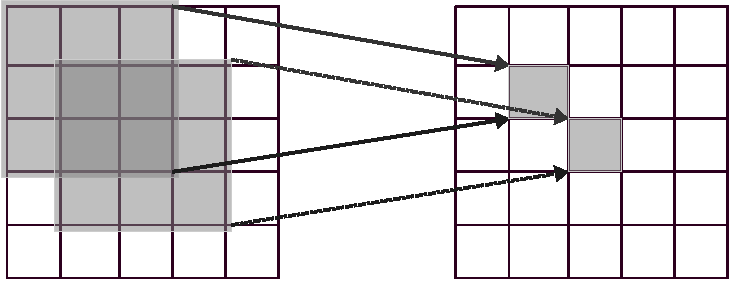
\includegraphics[width=0.8\textwidth]{pics/conv.pdf}
	\caption{Each individual neuron in the convolution layer (right matrix) connects to its receptive field using the same kernel. The value of the kernel is represented by the synaptic weights between the connected neurons.}
	\label{fig:conv}
\end{figure}

\section{Model Description}
\label{sec:mdc}
There are two CNNs proposed to accomplish the dynamic hand posture recognition task.
A straight forward method of template matching is employed at first, followed by a network of multi-layer perceptrons (MLP) trained to improve the recognition performance.


\begin{figure}
\centering
	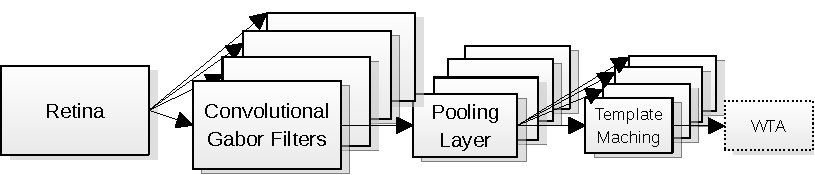
\includegraphics[width=0.8\textwidth]{pics/model1.pdf}
	\caption{Model 1. 
	The retina input is convolved with Gabor filters in the second layer, and then shrinks the sizes in the pooling layer.
	The templates are considered as convolution kernels in the last layer.
	The WTA circuit can be used as an option to show the template matching result more clearly.
	}
	\label{fig:model1}
\end{figure}
%\subsubsection{Model 1. Template Matching}

Model 1: Template Matching. Shown in Figure~\ref{fig:model1} the first layer is the retina input, followed by the convolutional layer, where the kernels are Gabor filters responding to edges of four orientations.
The third layer is the pooling layer where the size of the populations shrinks. 
This down-sampling enables robust classification due to its tolerance to variations in the precise shape of the input. 
The fourth layer is another convolution layer where the output from the pooling layer is convolved with the templates.
The optional layer of Winner-Take-All (WTA) neurons enables a clearer classification result due to the inhibition between the neurons.
In the Matlab simulation, the retina input spikes are buffered into 30~ms frames, and the neurons are simple linear perceptrons.
The templates are chosen by sampling the output of the pooling layer when given some reference stimulus, see Figure~\ref{fig:template}.

\begin{figure}
\centering
	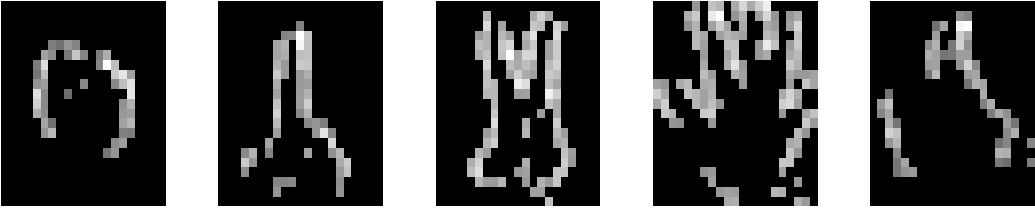
\includegraphics[width=0.8\textwidth]{pics/gesture.pdf}
	\caption{Templates of the five postures: `Fist',`Index Finger', `Victory Sign', `Full Hand' and `Thumb up'.}
	\label{fig:template}
\end{figure}

The Gabor filter is well-known as a linear filter for edge detection in image processing. 
A Gabor filter is a 2D convolution of a Gaussian kernel function and a sinusoidal plane wave; see Equation~\ref{equ:gabor}. 
\begin{equation}
\begin{array}{l}
\mathrm{Real Parts} = \exp \left(\frac{-x^{'2}+y^{'2}}{2\sigma ^{2}}\right)\cos \left(2\pi\frac{{x}'}{\lambda }\right)
\\
\\
\mathrm{Imaginary Parts} = \exp \left(\frac{-x^{'2}+y^{'2}}{2\sigma ^{2}}\right)\sin \left(2\pi\frac{{x}'}{\lambda }\right)
\\
\\
\mathrm{where:}
\\
\\
{x}'=x\cos (\theta ) + y\sin (\theta)
\\
\\
{y}'=-x\sin (\theta ) + y\cos (\theta)
\end{array}
\label{equ:gabor}
\end{equation}
$\theta$ represents the orientation of the filter, $\lambda$ is the wavelength of the sine wave, and $\sigma$ is the standard deviation of the Gaussian envelope. 
The frequency and orientation features are similar to the responses of V1 neurons in the human visual system. 
Only the real parts of the Gabor filters (see Figure~\ref{fig:gabor}) are used as the convolutional kernels to configure the weights between the input layer and the Gabor filter layer.

\begin{figure}
\centering
	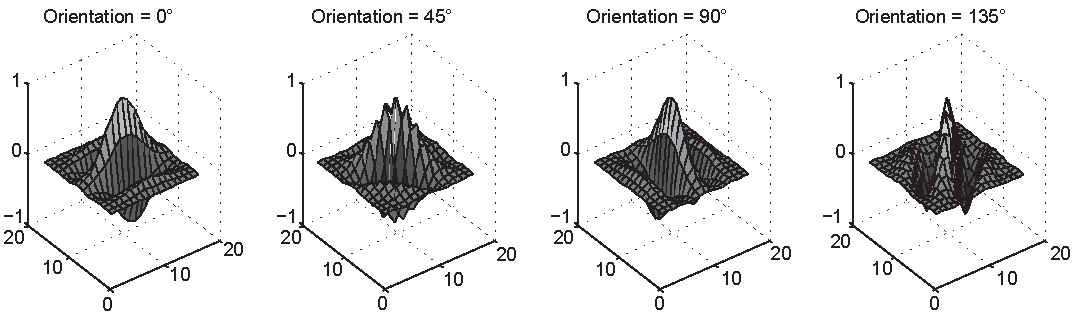
\includegraphics[width=0.8\textwidth]{pics/gabor.pdf}
	\caption{Real parts of the Gabor filters orienting four directions.}
	\label{fig:gabor}
\end{figure}

%The templates (see Figure~\ref{fig:template}) are manually selected from the output of the pooling layer in the framed Matlab simulation. 
The output score of a convolution is determined by the matching degree between the input and the kernel.
Regarding the template matching layer, each neuron in a population responds to how closely its receptive field matches the specific template.
The position of moving gesture is also naturally encoded in the address of template matching neuron.
Thus, there are five populations of template matching neurons, one for each hand posture listed.

%\subsubsection{Model 2. Trained MLP}
Model 2: Trained MLP. 
Inspired by the research of Lecun~\cite{lecun1998gradient}, we designed a combined network model with MLP and CNN (Figure~\ref{fig:model2}). 
The first three layers are exactly the same as the previous model.
The training images for the 3-layered MLP are of same size and the posture is centred in the images.
Therefore, a tracking layer plays an important role to find the most active region and forward the centred image to the next layer.

\begin{figure}
\centering
	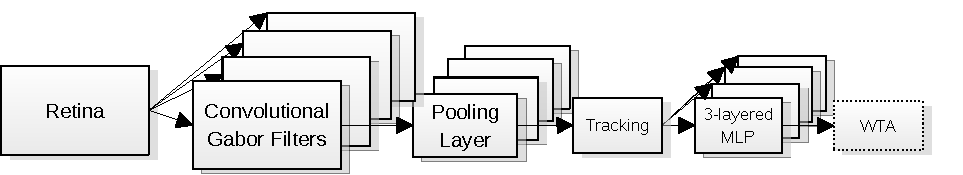
\includegraphics[width=0.8\textwidth]{pics/model2.pdf}
	\caption{Model 2. 
	The retina input convolves with Gabor filters in the second layer, and then shrinks the sizes in the pooling layer.
	The following tracking layer finds the most active area of some fixed size, moves the posture to the centre and pushes the image to the trained MLP.
	The winner-take-all (WTA) layer can be used as an option to show the template matching result more clearly.}
	\label{fig:model2}
\end{figure}

%Since the size of the input image of the MLP training is fixed and the position is centered, tracking plays a very important role to spot the valid region. 
%Tracking is naturally embedded in the pooling layer of the convolutional network, for the active neurons directly point out the lively receptive field. 

\section{Experimental Set-up}
\label{sec:tat}
In order to evaluate the cost and performance trade-offs in optimizing the number of neural components, both the convolutional models described above are tested at different scales. 
Five videos of every posture are captured from the silicon retina in AER format, all of similar size and moving clock-wise in front of the retina. 
The videos are cut into frames (30~ms per frame) and presented to the convolutional networks. 
The configurations of the networks are listed in Table~\ref{tbl:nns}.
The integration layer is not necessary in a convolutional network, but is used here to decrease the number of synaptic connections.

\begin{table}
\caption{Sizes of the convolutional neural networks.}
	\begin{subtable}{0.6\textwidth}
		
		\centering
		\caption{Model 1: Template matching}
		\begin{tabular}{p{0.26\textwidth}|p{0.3\textwidth}<{\centering}|p{0.26\textwidth}<{\centering}|p{0.26\textwidth}<{\centering}|p{0.26\textwidth}<{\centering}}
		%Line 1
		\Xhline{1.2pt}
		    & \multicolumn{2}{c|}{\tabincell{c}{\textbf{Full Resolution } \\\textbf{128 $\times$ 128}}}  
		    & \multicolumn{2}{c}{\tabincell{c}{\textbf{Sub-sampled Resolution} \\\textbf{32 $\times$ 32}}}
		    \\ \cline{2-5}
		%Line 2
			& \tabincell{c}{Population \\ Size}
			& \tabincell{c}{Connections \\ per Neuron}
			& \tabincell{c}{Population \\ Size}
			& \tabincell{c}{Connections \\ per Neuron}
			\\ \Xhline{1.2pt}
		%Line 3
		\tabincell{l}{\textbf{Retinal} \\\textbf{Input}}
			& 128 $\times$ 128	& 1	& 32 $\times$ 32	& 4 $\times$ 4
			\\ \hline
		%Line 4
		\tabincell{l}{\textbf{Gabor} \\\textbf{Filter}}
			& 112$\times$112$\times$4	& 17 $\times$ 17	& 28$\times$28$\times$4	& 5 $\times$ 5
			\\ \hline
		%Line 5
		\tabincell{l}{\textbf{Pooling} \\\textbf{Layer}}
			& 36$\times$36$\times$4	& 5 $\times$ 5	& null	& null
			\\ \hline
		%Line 6
		\tabincell{l}{\textcolor[rgb]{0.55,0.55,0.55}{\textbf{Integration}} \\ \textcolor[rgb]{0.55,0.55,0.55}{\textbf{Layer}}}
			& 36 $\times$ 36	& 4	& 28 $\times$ 28	& 4
			\\ \hline
		%Line 7
		\tabincell{l}{\textbf{Template} \\\textbf{Matching}}
			& 16$\times$16$\times$5	& 21 $\times$ 21	& 14$\times$14$\times$5	& 15 $\times$ 15
			\\ \Xhline{1.2 pt}
		%Line 8
		\textbf{Total}
			& $74,320$	& $15,216,512$	& $5,925$	& $318,420$
			\\ \Xhline{1.2 pt}
		\end{tabular}
		\label{tbl:m1}
	\end{subtable}
	\par\bigskip
	\begin{subtable}{0.6\textwidth}
		
		\centering
		\caption{Model 2: Trained MLP}
		\begin{tabular}{p{0.26\textwidth}|p{0.3\textwidth}<{\centering}|p{0.26\textwidth}<{\centering}|p{0.26\textwidth}<{\centering}|p{0.26\textwidth}<{\centering}}
		%Line 1
		\Xhline{1.2pt}
		    & \multicolumn{2}{c|}{\tabincell{c}{\textbf{Full Resolution} \\\textbf{128 $\times$ 128}}}  
		    & \multicolumn{2}{c}{\tabincell{c}{\textbf{Sub-sampled Resolution} \\\textbf{32 $\times$ 32}}}
		    \\ \cline{2-5}
		%Line 2
			& \tabincell{c}{Population \\ Size}
			& \tabincell{c}{Connections \\ per Neuron}
			& \tabincell{c}{Population \\ Size}
			& \tabincell{c}{Connections \\ per Neuron}
			\\ \Xhline{1.2pt}
		%Line 3
		\tabincell{l}{\textbf{Tracked} \\\textbf{Input}}
			& 21 $\times$ 21	& null	& 15 $\times$ 15	& null
			\\ \hline
		%Line 4
		\tabincell{l}{\textbf{Hidden} \\\textbf{Layer}}
			& 10	& 21$\times$21$\times$10	& 10	& 15$\times$15$\times$10
			\\ \hline
		%Line 5
		\tabincell{l}{\textbf{Recognition} \\\textbf{Layer}}
			& 5	& 5$\times$10	& 5	& 5$\times$10
			\\ \Xhline{1.2pt}
		%Line 6
		\textbf{Total}
			& $456$	& $4,460$	& $240$	& $2,300$
			\\ \Xhline{1.2 pt}
		\end{tabular}
		\label{tbl:m2}
	\end{subtable}
	\label{tbl:nns}
\end{table}

\section{Experimental Results}
\label{sec:exp}

\begin{figure}
\centering
	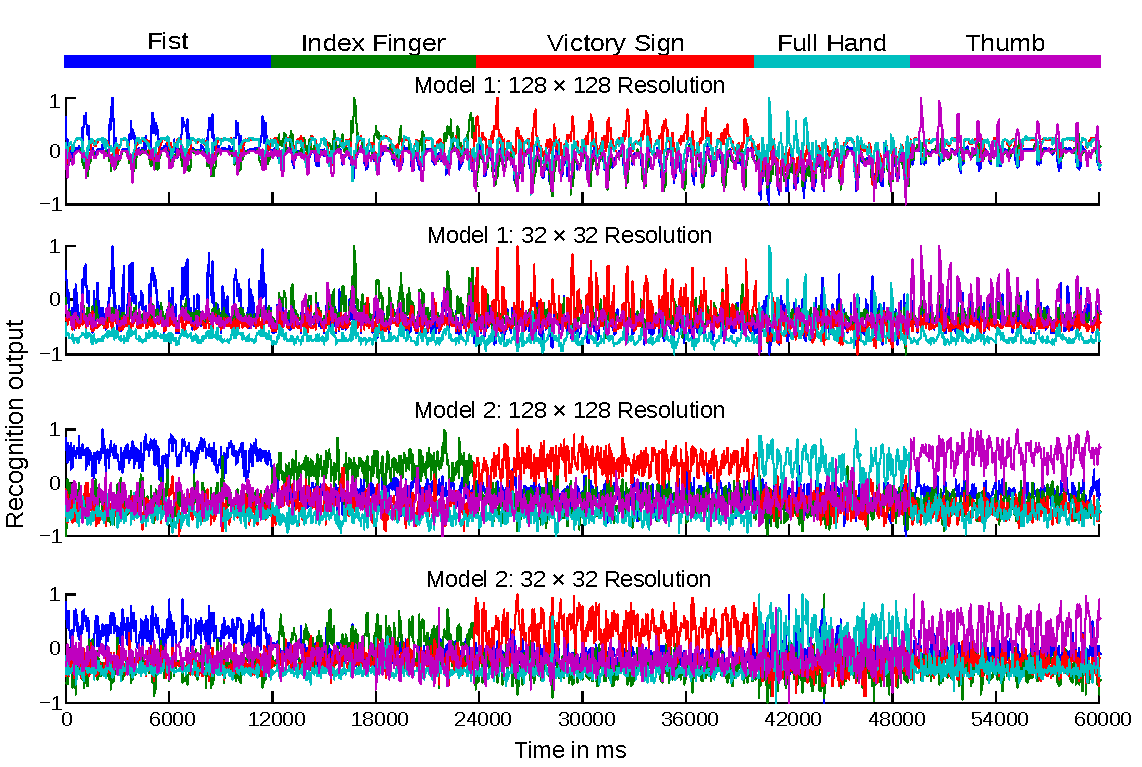
\includegraphics[width=0.8\textwidth]{pics/rateMatlab.pdf}
	\caption{Neural responses with time of four experiments to the same recorded moving postures.
	The recognition output is normalised to \mbox{[-1, 1]}.
	Every point represents the highest response in a specific population (different colour) for a 30~ms frame.
	The 1st plot refers to Model 1 with the full input resolution, and the 2nd plot Model 1 with the sub-sampled input resolution; and the 3rd and fourth plots both refer to Model 2, and with high and low input resolution respectively. 
	}
	\label{fig:matlabrec}
\end{figure}




In Figure~\ref{fig:matlabrec} the first two plots refer to Model 1, using template matching. Each colour represents one of the recognition populations. 
Each point in the plot is the highest neuronal response in the recognition population during the time of one frame (30~ms). 
The neuronal response, `the spiking rate', is normalised to [-1, 1]. 
It can be seen that the higher resolution input makes the boundaries between the classes clearer. 
On the other hand, recognition only happens when the test image and template are similar enough. 
The templates are only selected from the frames where the gestures are moving towards the right, and the gestures are moving clockwise in the videos, thus, all the peaks in plot 1 correspond with moments when the gesture moves towards right.  
It is notable that the higher resolution causes the recogniser to be more sensitive to the differences between the test data and the template, while the smaller neural network can recognize more generalized patterns. 
Therefore, a threshold is required to differentiate between data that is close enough and that which is not. 
Since the gestures are moving in four different directions during the clockwise movement, a rejection rate (i.e. none of the template is matched) of 75\% is to be expected. 

The latter two plots of Figure~\ref{fig:matlabrec} refer to Model 2. 
The three-layer MLP network significantly improves the recognition rate and can generalise the pattern. 
There is no rejection rate for Model 2, since the MLP is trained with all the moving directions of the postures.

Detailed results are listed in Table~\ref{tbl:rsl}. 
The correct recognition rate is calculated from the non-rejected frames.
The lower resolution of the 32$\times$32 retina input is adequate (85.83\%) for this gesture recognition task. 
The smaller network uses only 1/10th the number of neurons and 1/50th the number of synaptic connections compared with the full resolution network, while the recognition rate drops only around by 9.0\% with Model 1 and 17.2\% with Model 2.

\begin{table}
\centering
\caption{Recognition results using linear perceptrons in \%}
	\begin{tabular}{p{0.15\textwidth}|p{0.1\textwidth}<{\centering}|p{0.11\textwidth}<{\centering}|p{0.11\textwidth}<{\centering}|p{0.11\textwidth}<{\centering}|p{0.11\textwidth}<{\centering}}
		%Line 1
		\Xhline{1.2pt}
		    \multicolumn{2}{c|}{}	& \multicolumn{2}{c|}{\textbf{Model 1}}  
		    & \multicolumn{2}{c}{\textbf{Model 2}}
		    \\ \cline{3-6}
		%Line 2
		\multicolumn{2}{c|}{}	& \tabincell{c}{High \\ Resolution}
			& \tabincell{c}{Low \\ Resolution}
			& \tabincell{c}{High \\ Resolution}
			& \tabincell{c}{Low \\ Resolution}
			\\ \Xhline{1.2pt}
		%Line 3-4	
		\multirow{2}{*}{\tabincell{l}{\textbf{Fist}\\ (399 Frames)}}
			& Correct & 99.11	& 99.23	& 96.24	& 84.21
			\\ \cline{2-6}
			& Reject  & 71.93 & 67.42 	& Null	& Null
			\\ \hline
		%Line 5-6
		\multirow{2}{*}{\tabincell{l}{\textbf{Index Finger} \\ (392 Frames)}}
			& Correct & 92.98	& 80.00	& 94.39	& 71.69
			\\ \cline{2-6}
			& Reject & 70.92	& 75.77 	& Null	& Null
			\\ \hline
		%Line 7-8
		\multirow{2}{*}{\tabincell{l}{\textbf{Victory Sign} \\ (551 Frames)}}
			& Correct & 96.56	& 93.07	& 95.64	& 87.66
			\\ \cline{2-6}
			& Reject & 73.68	& 81.67 	& Null	& Null
			\\ \hline
		%Line 9-10
		\multirow{2}{*}{\tabincell{l}{\textbf{Full Hand} \\ (293 Frames)}}
			& Correct & 95.65	& 72.41	& 93.52	& 72.01
			\\ \cline{2-6}
			& Reject & 92.15	& 90.10 	& Null	& Null
			\\ \hline
		%Line 10-11
		\multirow{2}{*}{\tabincell{l}{\textbf{Thumb up} \\ (391 Frames)}}
			& Correct & 89.61	& 84.44	& 96.68	& 74.68
			\\ \cline{2-6}
			& Reject & 80.31	& 76.98 	& Null	& Null
			\\ \hline\hline
		\multirow{2}{*}{\tabincell{l}{\textbf{Average}}}
			& Correct & 94.78	& 85.83	& 95.29	& 78.05
			\\ \cline{2-6}
			& Reject & 77.80	& 78.39 	& Null	& Null
			\\ \hline
	\end{tabular}
	\label{tbl:rsl}
\end{table}


\chapter{Recognition on SpiNNaker}
\label{cha:rsp}

\section{Moving from Perceptrons to Spiking Neurons}
It remains a challenge to transform traditional artificial neural networks into spiking ones.
There are attempts~\cite{la2008response}~\cite{burkitt2006review} to estimate the output firing rate of the LIF neurons (Equation~\ref{equ:lif}) under certain conditions. 
%For the model illustrated above, there are two types of synaptic connection: one-to-one connections in the retina layer and N-to-one connections in all the convolutional layers (the pooling layer is also included). 
%For the retina layer, 1) the problem is: what is the connection weight between two single LIF neurons to make a post-synaptic neuron fire whenever the pre-synaptic neuron generates a spike? 
%While for the convolutional neurons, 2) given the input spike rates, LIF neuron parameters and the output spiking rate, what are the corresponding weights between the two layers?
\begin{equation}
\frac{\D \: V(t)}{\D\:  t}=-\frac{V(t)-V_\mathit{rest}}{\tau_m}+\frac{I(t)}{C_m}
\label{equ:lif}
\end{equation}
The membrane potential $V$ changes in response to input current $I$, starting at the resting membrane potential  $V_{rest}$, where the membrane time constant is $\tau_m = R_mC_m$, $R_m$ is the membrane resistance and $C_m$ is the membrane capacitance.

Given a constant current injection $I$, the response function, i.e. firing rate, of the LIF neuron is
\begin{equation}
\lambda_\mathit{out}=
\left [ t_\mathit{ref}-\tau_m\ln \left ( 1-\frac{V_{th}-V_\mathit{rest}}{IR_m}  \right )\right ]^{-1}
\label{equ:consI}
\end{equation}
when $IR_m>V_{th}-V_{rest}$, otherwise the membrane potential cannot reach the threshold $V_{th}$ and the output firing rate is zero. 
The absolute refractory period $t_\mathit{ref}$ is included, where all input during this period is invalid.
In a more realistic scenario, the post-synaptic potentials (PSPs) are triggered by the spikes generated from the neuron's pre-synaptic neurons other than a constant current.
Assume that the synaptic inputs are Poisson spike trains, the membrane potential of the LIF neuron is considered as a diffusion process. Equation~\ref{equ:lif} can be modelled as a stochastic differential equation referring to Ornstein-Uhlenbeck process,
\begin{equation}
\tau_m\frac{\D\:V(t)}{\D\:  t}=-\left[V(t)-V_\mathit{rest}\right] + \mu + \sigma\sqrt{2\tau_m}\xi (t)
\label{equ:sde}
\end{equation}
where
\begin{equation}
\begin{array}{l}
\mu=\tau_m(\mathbf{w_E\cdot\lambda_E}-\mathbf{w_I\cdot\lambda_I})
\\
\\
\sigma ^{2} = \frac{\tau_m}{2}\left(\mathbf{w_E^{2}\cdot\lambda_E}+\mathbf{w_I^{2}\cdot\lambda_I}\right)
\end{array}
\label{equ:ou}
\end{equation}
are the conditional mean and variance of the membrane potential.
The delta-correlated process $\xi(t)$ is Gaussian white noise with zero mean, $\mathbf{w_E}$ and $\mathbf{w_I}$ stand for the weight vectors of the excitatory and the inhibitory synapses, and $\mathbf{\lambda}$ represents the vector of the input firing rate.
The response function of the LIF neuron with Poisson input spike trains is given by the Siegert function~\cite{siegert1951first}, 
\begin{equation}
\lambda_\mathit{out}=\left(\tau_\mathit{ref} + \frac{\tau_Q}{\sigma_Q}\sqrt{\frac{\pi}{2}} \int_{V_\mathit{rest}}^{V_\mathit{th}}du \:\exp \left(\frac{u-\mu_Q}{\sqrt2\sigma_Q} \right )^{2}\left[1+erf \left(\frac{u-\mu_Q}{\sqrt2\sigma_Q} \right ) \right ]\right)^{-1}
%\begin{split}
%\lambda_\mathit{out}=\left(\tau_\mathit{ref} + \frac{\tau_Q}{\sigma_Q}\sqrt{\frac{\pi}{2}} \int_{V_\mathit{rest}}^{V_\mathit{th}}\D u \:\exp \left(\frac{u-\mu_Q}{\sqrt2\sigma_Q} \right )^{2}\left[1+\mathrm{erf} \left(\frac{u-\mu_Q}{\sqrt2\sigma_Q} \right ) \right ]\right)^{-1}
%\end{split}
%\label{equ:sgt}
\end{equation}
%\begin{align}
%\lambda_\mathit{out} &=\left(\tau_\mathit{ref} + \frac{\tau_Q}{\sigma_Q}\sqrt{\frac{\pi}{2}} \int_{V_\mathit{rest}}^{V_\mathit{th}}\D\,u \:\exp \left(\frac{u-\mu_Q}{\sqrt2\sigma_Q} \right )^{2} \right. \nonumber \\
%&\qquad \left. \vphantom{\int_t} \cdot  \left[1+\mathrm{erf} \left(\frac{u-\mu_Q}{\sqrt2\sigma_Q} \right ) \right ]\right)^{-1}
%\label{equ:sgt}
%\end{align}
where $\tau_Q, \mu_Q, \sigma_Q$ are identical to $\tau_m, \mu, \sigma$ in Equation~\ref{equ:ou}, and erf is the error function.

Still there are some limitations on the response function. 
For the diffusion process, only small amplitude (weight) of the PostSynaptic Potentials (PSPs) generated by a large amount of input spikes (high spiking rate) work under this circumstance; 
plus, the delta function is required, i.e. the synaptic time constant is considered to be zero. Thus only a rough approximation of the output spike rate has been determined.
Secondly, given different input spike rate to each pre-synaptic neurons, the parameters of the LIF neuron and the output spiking rate, how to tune every single corresponding synaptic weight remains a difficult task.


\section{Live Recognition}
\begin{figure}[h!]
	\centering
	\begin{subfigure}[t]{0.48\textwidth}
		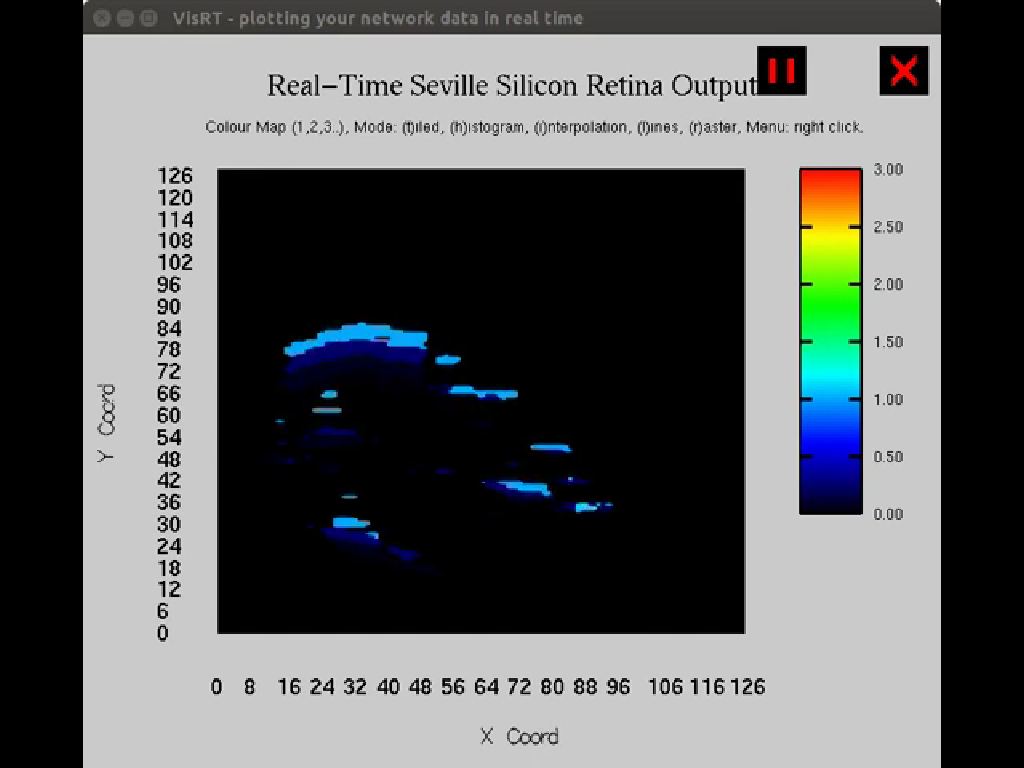
\includegraphics[width=\textwidth]{pics/live1_colour.png}
		\caption{Neural responses of the Gabor filter layer orienting to the horizontal direction~\cite{video1} }
		\label{fig:live1}
	\end{subfigure}
	\begin{subfigure}[t]{0.48\textwidth}
		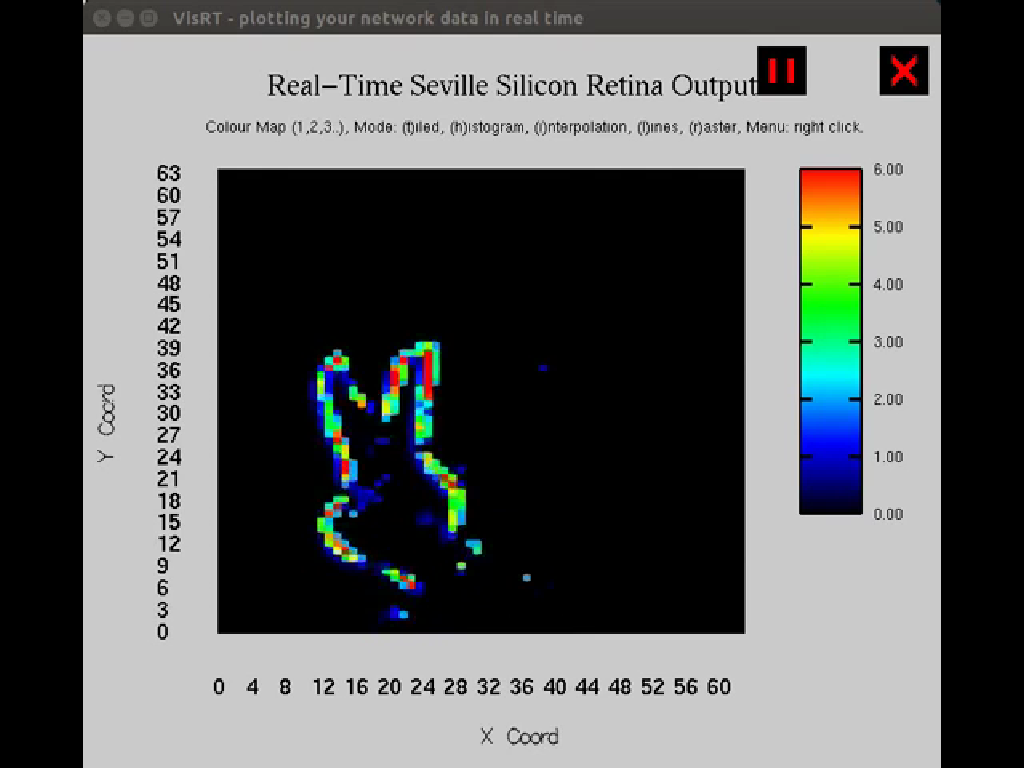
\includegraphics[width=\textwidth]{pics/live2_colour.png}
		\caption{Neural responses of the integrate layer~\cite{video2}}
		\label{fig:live2}
	\end{subfigure}
	\\
	\begin{subfigure}[t]{\textwidth}
		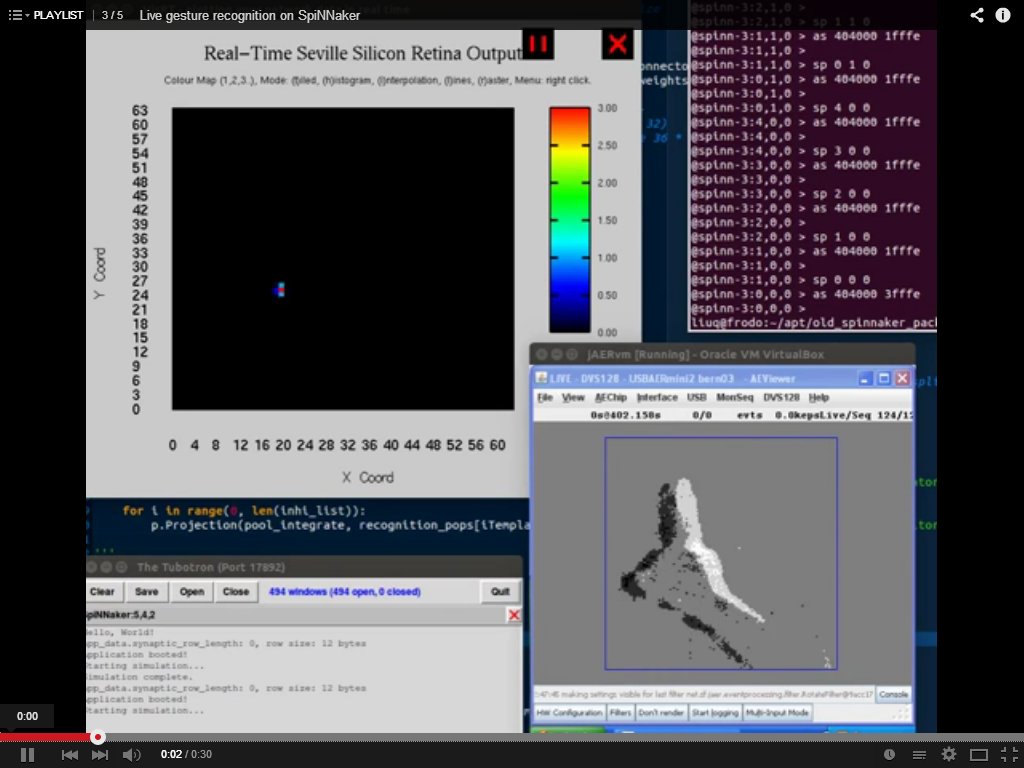
\includegraphics[width=\textwidth]{pics/live_colour.png}
		\caption{Snapshot of the neuron responses of the template matching layer~\cite{video3}}
		\label{fig:live3}
	\end{subfigure}	
	
	\caption{Snapshots of the real-time dynamic posture recognition system on SpiNNaker.
	}
	\label{fig:live}
\end{figure}
We implemented the prototype of the dynamic posture recognition system on SpiNNaker using LIF neurons. 
The input retina layer consists of 128$\times$128 neurons; 
each Gabor filter has 112$\times$112 valid neurons, since the kernel size is 17$\times$17; 
each pooling layer is as big as 36$\times$36, convolving with five template kernels (21$\times$21); 
thus, the recognition populations are 16$\times$16 neurons each. Altogether $74,320$ neurons and $15,216,512$ synapses, use up to 19 chips (290 cores) on a 48-node board, see Table~\ref{tbl:m1}. Regarding the lower resolution of 32$\times$32 retinal input, the network (Table~\ref{tbl:m2}) consists of $5,925$ neurons and $318,420$ synapses taking up only two chips (31 cores) of the board.

Figure~\ref{fig:live} shows snapshots of neural responses of some populations during real-time recognition.
Figure~\ref{fig:live1} is a snapshot of the Gabor population which prefers the horizontal direction, given the input posture of a `Fist'; and Figure~\ref{fig:live2} shows the activity of the neurons in the integration layer, given a 'Victory Sign'.
And the active neurons in the visualiser in Figure~\ref{fig:live3} are pointing out the position of the recognised pattern the `Index finger'. 
All the supporting demonstrative videos can be found on YouTube~\cite{video1, video2, video3}. %\footnote{\url{
%https://www.youtube.com/watch?v=PvJy6RKAJhw&feature=youtu.be&list=PLxZ1W-Upr3eoQuLxq87qpUL-CwSphtEBJ, http://youtu.be/FZJshPCJ1pg?list=PLxZ1W-Upr3eoQuLxq87qpUL-CwSphtEBJ, http://youtu.be/yxN90aGGKvg?list=PLxZ1W-Upr3eoQuLxq87qpUL-CwSphtEBJ}}.


\section{Recognition of Recorded Data}
To compare with the results of the experiments carried out with Matlab (in Section~\ref{sec:exp}), the same recorded retinal data is conducted into SpiNNaker.
Only Model 1 is tested on the neuromorphic hardware platform, since tracking is still need to investigate using SNN (for Model 2) in the future. 
The recorded data is presented as spike source array in the system with 128$\times$128 input (see Figure~\ref{fig:ssa}) while the data is forwarded to a sub-sampling layer of 32$\times$32 resolution in the system of the smaller network (see Figure~\ref{fig:ssa32}). 
The output spikes generated from the recognition populations with time are shown in Figures~\ref{fig:rps} and \ref{fig:rps32} for full resolution and lower systems respectively. 
More spikes are generated during the period when the preferred input posture is shown. 


\begin{figure}[h!]
\centering
	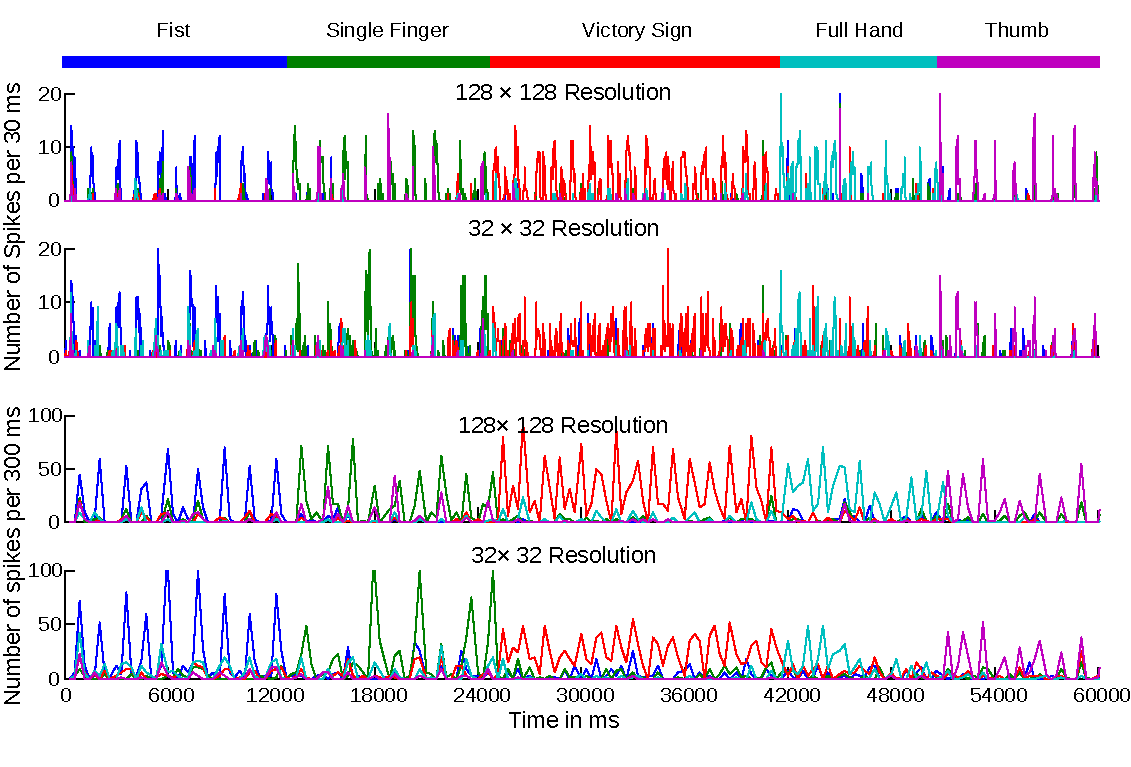
\includegraphics[width=\textwidth]{pics/rateSpiNN.pdf}
	\caption{Real-time neural responses of two experiments on SpiNNaker with time to the same recorded postures.
	These two experiments only differ in input resolution.
	The result of the high input resolution test is plotted the first with a sample frame of 30~ms; 
	while the 3rd plot shows the same result with a sample frame of 300~ms.
	The other two plots refer to the smaller input resolution.
	Every point represents the over all number of spikes of a specific population (different colour) in a `frame'.
	}
	\label{fig:spikerec}
\end{figure}

Correspondingly, the spiking rates of each recognition population is sampled into frames (Figure~\ref{fig:spikerec}) to make a comparison with the Matlab simulation. 
Each colour represents one recognition population, and the spike activity goes higher when the input posture matches the template. 
Firstly, the spike rates are sampled into 30~ms frames which is in accordance with the Matlab experiments.
In the Matlab simulation, the templates are trained with cut frames and so the test images are also fixed to the same length frames.
Otherwise, the recogniser will not work properly because of the replications of the moving posture.
Contrasting this, the spiking rates can be sampled to various frame lengths.
Thus, the other two plots in the figure illustrate the classification in a wider window of 300~ms.
From Table~\ref{tbl:srr}, the recognition and rejection rates are quantified as percentages.

\begin{table}[h!]
	\centering
	\caption{Real-time recognition results on SpiNNaker in \%}
	\begin{tabular}{p{0.15\textwidth}|p{0.1\textwidth}<{\centering}|p{0.11\textwidth}<{\centering}|p{0.11\textwidth}<{\centering}|p{0.11\textwidth}<{\centering}|p{0.11\textwidth}<{\centering}}
		%Line 1
		\Xhline{1.2pt}
		\multicolumn{2}{c|}{}	& \multicolumn{2}{c|}{\textbf{30~ms per frame}}  
		& \multicolumn{2}{c}{\textbf{300~ms per frame}}
		\\ \cline{3-6}
		%Line 2
		\multicolumn{2}{c|}{}	& \tabincell{c}{High \\ Resolution}
		& \tabincell{c}{Low \\ Resolution}
		& \tabincell{c}{High \\ Resolution}
		& \tabincell{c}{Low \\ Resolution}
		\\ \Xhline{1.2pt}
		%Line 3-4	
		\multirow{2}{*}{\tabincell{l}{\textbf{Fist}}}
		& Correct & 91.78	& 78.02	& 100	& 92.31
		\\ \cline{2-6}
		& Reject  & 82.78 & 78.54 	& 70.73	& 68.29
		\\ \hline
		%Line 5-6
		\multirow{2}{*}{\tabincell{l}{\textbf{Index Finger}}}
		& Correct & 78.25	& 78.25	& 88.24	& 72.22
		\\ \cline{2-6}
		& Reject & 80.46	& 73.56 	& 57.50	& 55.00
		\\ \hline
		%Line 7-8
		\multirow{2}{*}{\tabincell{l}{\textbf{Victory Sign} }}
		& Correct & 96.48	& 86.27	& 95.00	& 92.50
		\\ \cline{2-6}
		& Reject & 64.46	& 72.68 	& 28.57	& 28.57
		\\ \hline
		%Line 9-10
		\multirow{2}{*}{\tabincell{l}{\textbf{Full Hand}}}
		& Correct & 85.29	& 60.78	& 90.00	& 75.00
		\\ \cline{2-6}
		& Reject & 67.31	& 83.65 	& 35.48	& 61.29
		\\ \hline
		%Line 10-11
		\multirow{2}{*}{\tabincell{l}{\textbf{Thumb up}}}
		& Correct & 84.09	& 88.10	& 91.67	& 100
		\\ \cline{2-6}
		& Reject & 87.54	& 73.81 	& 66.67	& 66.67
		\\ \hline\hline
		\multirow{2}{*}{\tabincell{l}{\textbf{Average}}}
		& Correct & 87.18	& 78.28	& 92.98	& 86.41
		\\ \cline{2-6}
		& Reject & 76.51	& 76.45 	& 51.79	& 55.96
		\\ \hline
	\end{tabular}
	\label{tbl:srr}
\end{table}

Comparing with the results of Matlab simulation (Table~\ref{tbl:rsl}), the recognition rate is about 7.6\% lower at both high and low resolutions, and the rejection rate remains the same slightly above 75\%. 
However, by changing the frame length to 300~ms recognition rates reach (93.0\% for the larger network) or exceed (86.4\% for smaller network ) the Matlab simulation, meanwhile the rejection rates also drop dramatically by 26.0\% and 22.4\%.
This is in accordance with natural visual responses, which means, the longer an object shows, the more accurate the recognition will be.
Between the two network scales there is also a smaller gap in recognition rates as the window length grows, i.e. 8.9\% and 6.6\% respectively.
%Considering the cost and performance trade-off, with only 1/10th resources required, the small network, is acceptable and can be even improved after applying tracking and learning.
%Regarding the latency between the retinal input and the recognition, we compared the spiking peak of the Matlab simulation and the real-time SpiNNaker test.
%The overall latency is about 1150~ms from a posture being shown to its recognition. 

\begin{figure}
\centering
	\begin{subfigure}[t]{0.4\textwidth}
		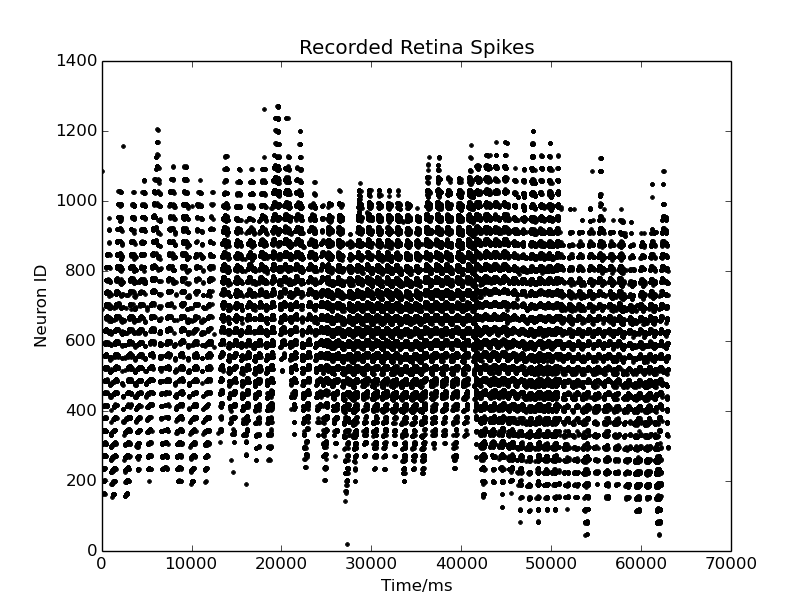
\includegraphics[width=\textwidth]{pics/figure_r.png}
	    \caption{Retinal input population }
	    \label{fig:ssa}
	\end{subfigure}
	\begin{subfigure}[t]{0.4\textwidth}
		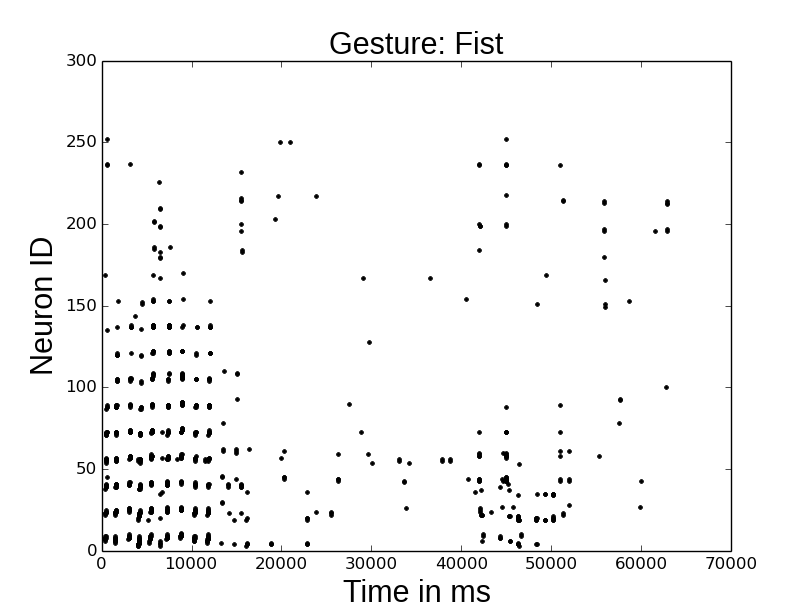
\includegraphics[width=\textwidth]{pics/figure_1.png}
		\caption{Template matching population, `Fist'}
	    \label{fig:rec0}
	\end{subfigure}
	\\
	\begin{subfigure}[t]{0.4\textwidth}
		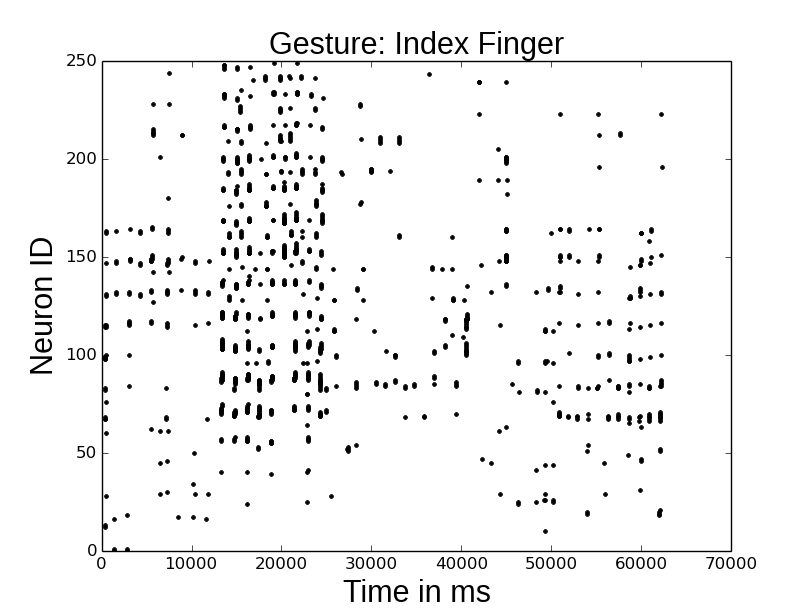
\includegraphics[width=\textwidth]{pics/figure_2.png}
		\caption{Template matching population, `Index Finger'}
	    \label{fig:rec1}
	\end{subfigure}	
	\begin{subfigure}[t]{0.4\textwidth}
		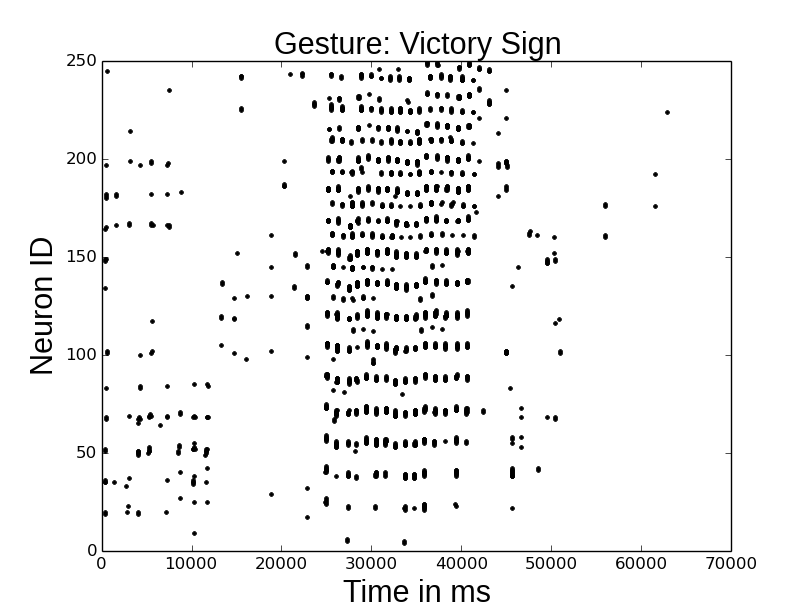
\includegraphics[width=\textwidth]{pics/figure_3.png}
		\caption{Template matching population, `Victory Sign'}
	\end{subfigure}	
	\\
	\begin{subfigure}[t]{0.4\textwidth}
		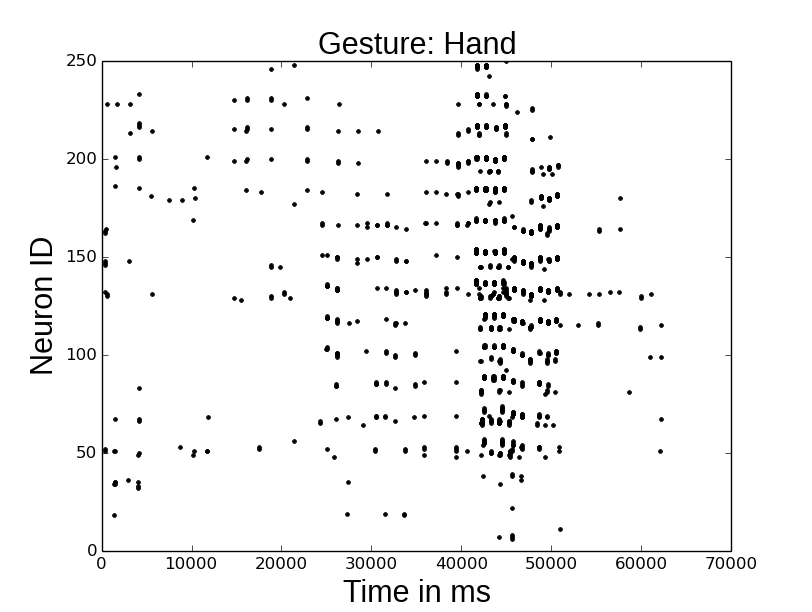
\includegraphics[width=\textwidth]{pics/figure_4.png}
		\caption{Template matching population, `Full Hand'}
	    \label{fig:rec5}
	\end{subfigure}	
	\begin{subfigure}[t]{0.4\textwidth}
		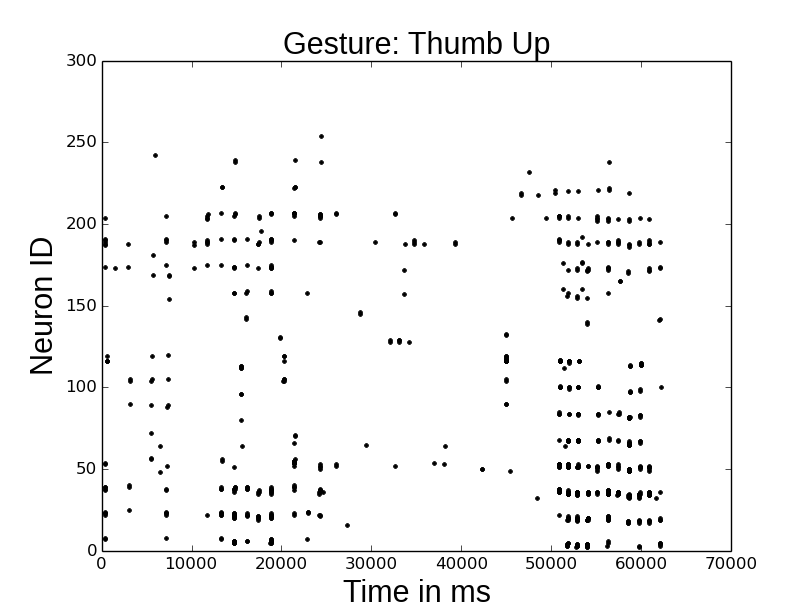
\includegraphics[width=\textwidth]{pics/figure_5.png}
		\caption{Template matching population, `Thumb Up'}
	    \label{fig:rect}
	\end{subfigure}	
\caption{Spikes captured during the live recognition of the recorded retinal input with the resolution of 128$\times$128. }
\label{fig:rps}
\end{figure}
\begin{figure}
\centering
	\begin{subfigure}[t]{0.4\textwidth}
		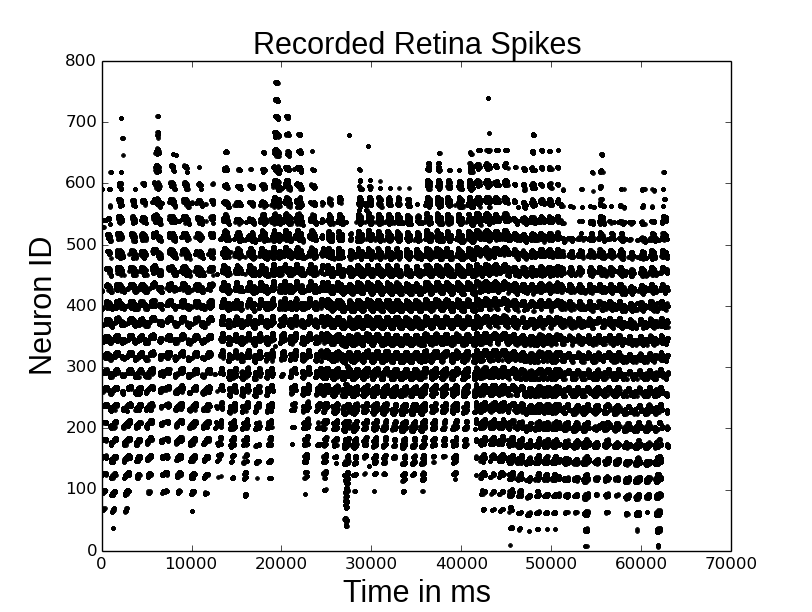
\includegraphics[width=\textwidth]{pics/figure_32_r.png}
	    \caption{Retinal input population }
	    \label{fig:ssa32}
	\end{subfigure}
	\begin{subfigure}[t]{0.4\textwidth}
		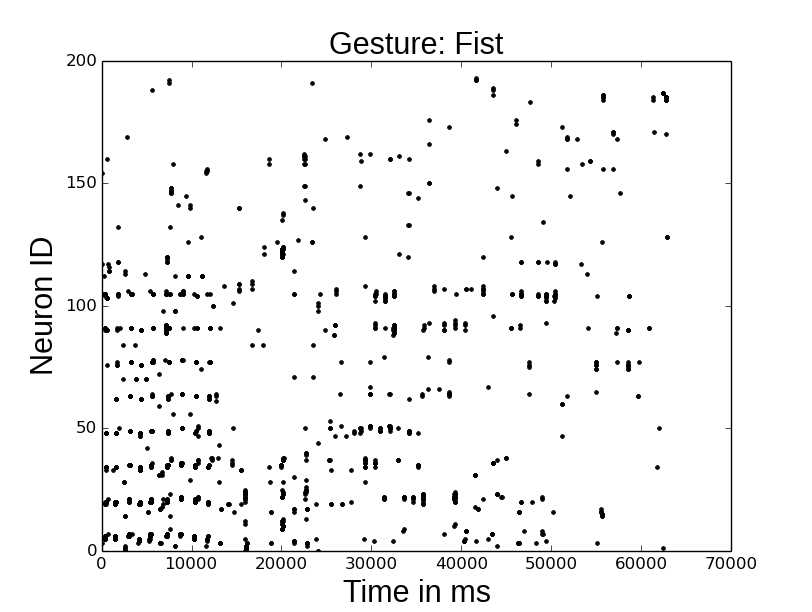
\includegraphics[width=\textwidth]{pics/figure_32_1.png}
		\caption{Template matching population, `Fist'}
	    \label{fig:rec032}
	\end{subfigure}
	\\
	\begin{subfigure}[t]{0.4\textwidth}
		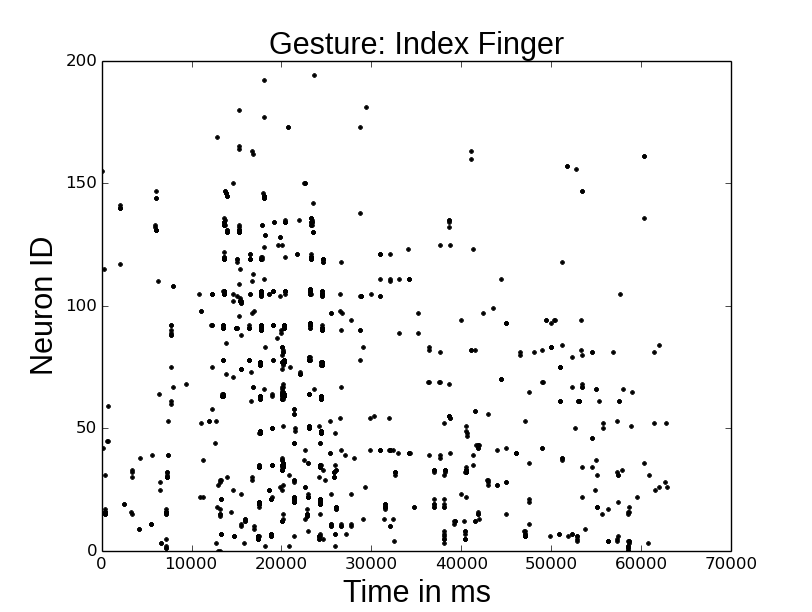
\includegraphics[width=\textwidth]{pics/figure_32_2.png}
		\caption{Template matching population, `Index Finger'}
	    \label{fig:rec132}
	\end{subfigure}	
	\begin{subfigure}[t]{0.4\textwidth}
		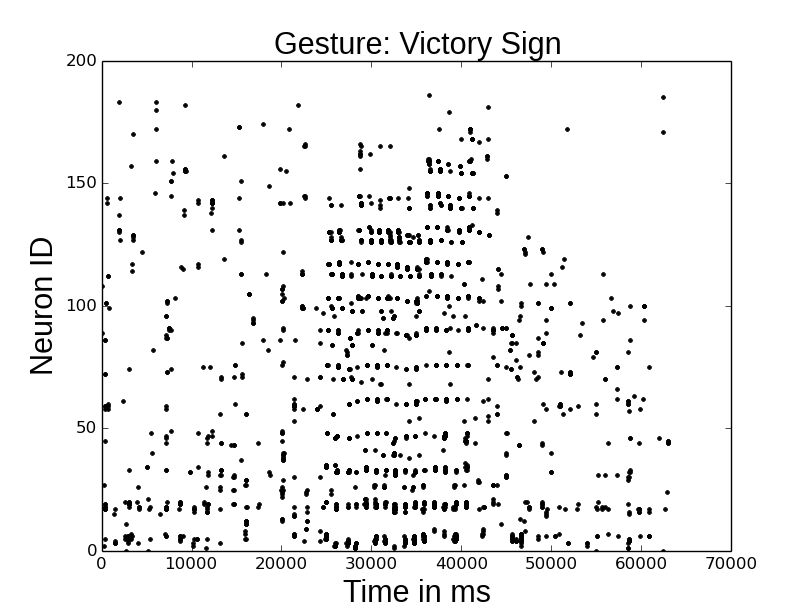
\includegraphics[width=\textwidth]{pics/figure_32_3.png}
		\caption{Template matching population, `Victory Sign'}
	\end{subfigure}	
	\\
	\begin{subfigure}[t]{0.4\textwidth}
		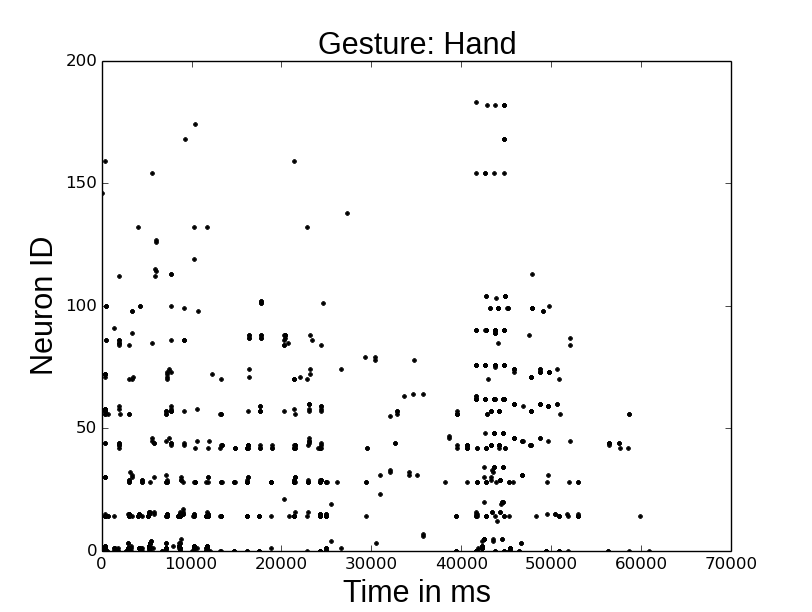
\includegraphics[width=\textwidth]{pics/figure_32_4.png}
		\caption{Template matching population, `Full Hand'}
	    \label{fig:rec532}
	\end{subfigure}	
	\begin{subfigure}[t]{0.4\textwidth}
		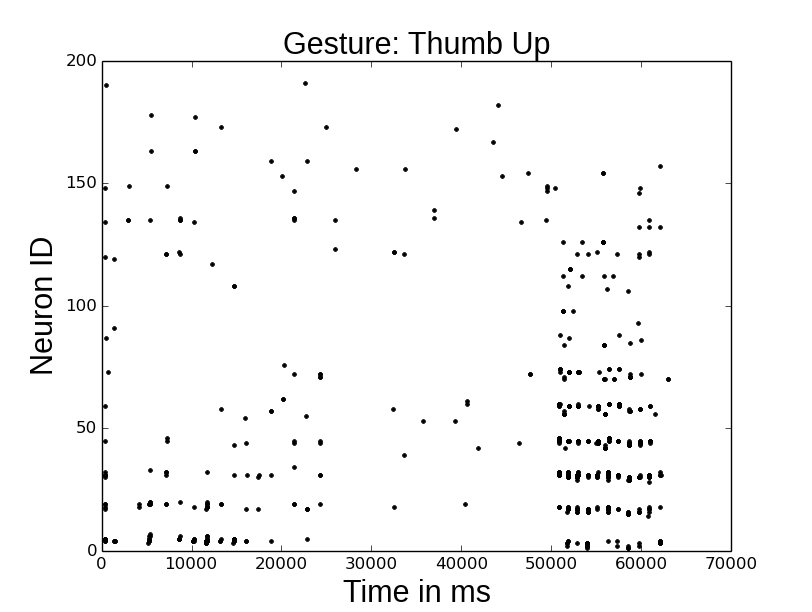
\includegraphics[width=\textwidth]{pics/figure_32_5.png}
		\caption{Template matching population, `Thumb Up'}
	    \label{fig:rect32}
	\end{subfigure}	
\caption{Spikes captured during the live recognition of the recorded retinal input with the resolution of 32$\times$32. }
\label{fig:rps32}
\end{figure}

\chapter{Contributions and Research Plan}
\label{cha:plan}
\section{Contributions}
%Motivation
To explore how brain may recognise objects in its general, accurate, invariant and energy-efficient manner, this work proposes the use of a neuromorphic hardware system which includes a DVS retina connected to SpiNNaker, a real-time SNN simulator.
%Problem
Building a hand gesture recognition system based on this bespoke hardware for dynamic hand postures is a first step in the study of the ventral visual pathway in the brain.
%Methods
Inspired by the structures of the primary visual cortex, convolutional neural networks are modelled, and the V1-like neurons are simulated with both linear perceptrons and LIF neurons.
This model is position invariant to recognise five hand postures.

%Results
%The larger network of 74,210 neurons and 15,216,512 synapses runs smoothly in real-time on SpiNNaker using 290 cores within a 48-node board.
%The smaller network using 1/10 of the resources is able to recognise the postures in real-time with an accuracy about 86.4\% in average, which is 
%only 6.6\% lower than the former but with a better cost/performance ratio.

The detailed contributions are listed below:
\begin{itemize}
	\item Modelling a convolutional neural network which can recognise moving postures (position invariant) with V1-like neurons.
	\item Translation of conventional artificial neural networks of perceptrons to spiking neural networks of LIF neurons using the Siegert function.
	\item Configuring the SpiNNaker neuromorphic platform to communicate with the silicon retina to perform real-time posture recognition using spiking neurons.
	\item Maintaining software to make SpiNNaker receive correct recorded spikes and compare performance with perceptrons and also visualise the live neural activity in real time.
\end{itemize}
	
%In this paper, we implement a dynamic hand posture recognition system running completely on a hardware neuromorphic platform.
%The SNN based classifier is able to recognise moving hand postures instead of static digit or face recognition proposed before.
%The network model is translated from linear perceptrons to LIF spiking neurons with a 10\% drop of accuracy in 30~ms windowing;
%while the performance reaches and even exceeds the perceptrons version when the window length is set to 300~ms.
%Various network sizes are configured to explore the cost and performance trade-off.
%In the tests of linear perceptrons the recognition rate of the smaller network is \% lower for the template matching model and \% lower for the trained MLP model.
%For the SNN based real-time experiments, both the larger network with $74,320$ LIF neurons and $15,216,512$ synapses, and the smaller network with 1/10 of the neurons and 1/50 of the synapses run smoothly on SpiNNaker.
%The gap of recognition rate narrows when the spiking rate is sampled into wider frame of 300~ms.
%The recognition rates of both linear perceptrons (\%) and spiking neurons (\%) with 32 $\times$ 32 input resolution are adequate for the recognition of the moving hand postures.
%This work is a good attempt to start exploring the visual process of the brain.

%Later, we will look more into the overall network latency, which could be due to the system latency and the performance of the rate coding. 
\section{Achievements }
\subsection{Publications}
\begin{itemize}

	\item Q. Liu and S. Furber, ``Real-time recognition of dynamic hand posture on a neuromorphic system." Artificial Neural Networks ICANN 2015. Springer Berlin Heidelberg. (Under review)


	\item Q. Liu, X. Lagorce, E. Stromatias, D. Emmanouilidou, R. Benosman, S. Furber and S. Liu, ``A large-scale, real-time sound localization on a neuromorphic platform." Neuromorphic Engineering. (Under proof reading of co-authors)

	\item Q. Liu, C. Patterson, S. Furber, Z. Huang, Y. Hou, and H. Zhang, ``Modeling populations of spiking neurons for fine timing sound localization." in Neural Networks (IJCNN), The 2013 International Joint Conference on, pp.1-8, Aug 2013.
\end{itemize}
\subsection{Workshops}
\begin{itemize}
	\item The 2014 CapoCaccia Cognitive Neuromorphic Engineering Workshop,\\ 28/04/2014 - 10/05/2014, Alghero, Sardinia, Italy 
	\item From Maps to Circuits: Models and Mechanisms for Generating Neural Connections, 28/07/2014 - 29/07/2014, Edinburgh UK
\end{itemize}
\section{Future Work} 
\begin{figure}[h!]
	\centering
	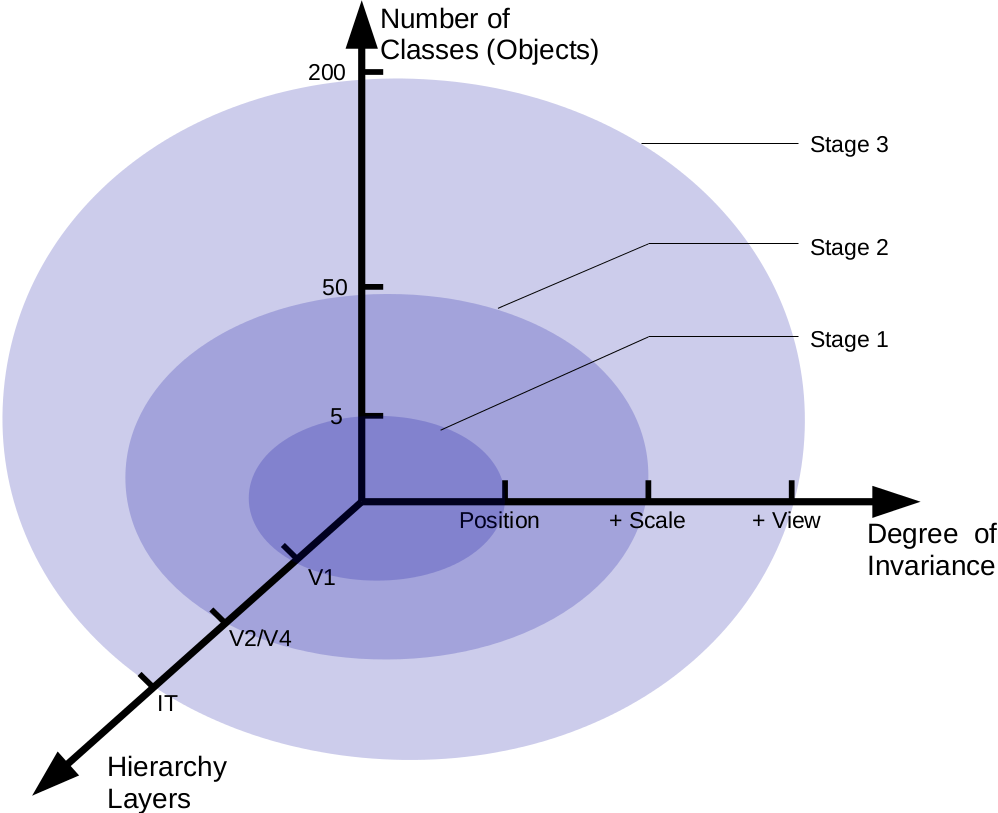
\includegraphics[width=0.75\textwidth]{pics/stages.png}
	\caption{3D representation of the research plan on the transformation-invariant object recognition system.
	Three milestones are pointed out indicating the expected targets of the object recognition networks.
	}
	\label{Fig:3Dplan}
\end{figure}
The proposed research plan is illustrated in Figure~\ref{Fig:3Dplan}, where the scope of the research is estimated in three dimensions.
To build a biologically-plausible object recognition system using spiking neurons, this work will be completed in three stages:
\begin{enumerate}
	\item Year 1, building a position-invariant object recognition system exploiting V1-like neurons to classify five hand postures. 
	\item Year 1.5, combining scale- with position-invariance on the object recognition system, and building the hierarchy ventral pathway to the V2/V4 layer to recognise 50 simple combined features such as gratings and contours.
	\item Year 2.5. integrating position-, scale- and view-invariance by modelling the hierarchical visual pathway up to the IT cortex and equipping the system with the ability to recognise 200 objects in real time.
\end{enumerate}
%The recognition ability of the system is measured in three dimensions: the hierarchy layers, degree of invariance and the network size.
 
This work will contribute to the understanding of biological visual processing by means of mimicking the neural activities in the ventral stream.
More importantly, the research will apply the accurate, rapid and robust approaches to artificial systems by exploring the brain's invariant object recognition.
The performance of the real-time recognition system will be tested on each milestone to validate the success of the models.
The neural activities and recognition rate will also be compared with biological data.

The key research steps are listed in Figure~\ref{Fig:gantt}.
Since the incremental work flow is hard to present in Gantt charts, only the work for the first milestone is shown.
The subsequent sections will outline the key research stages.



\begin{figure}[h!]
	\centering
	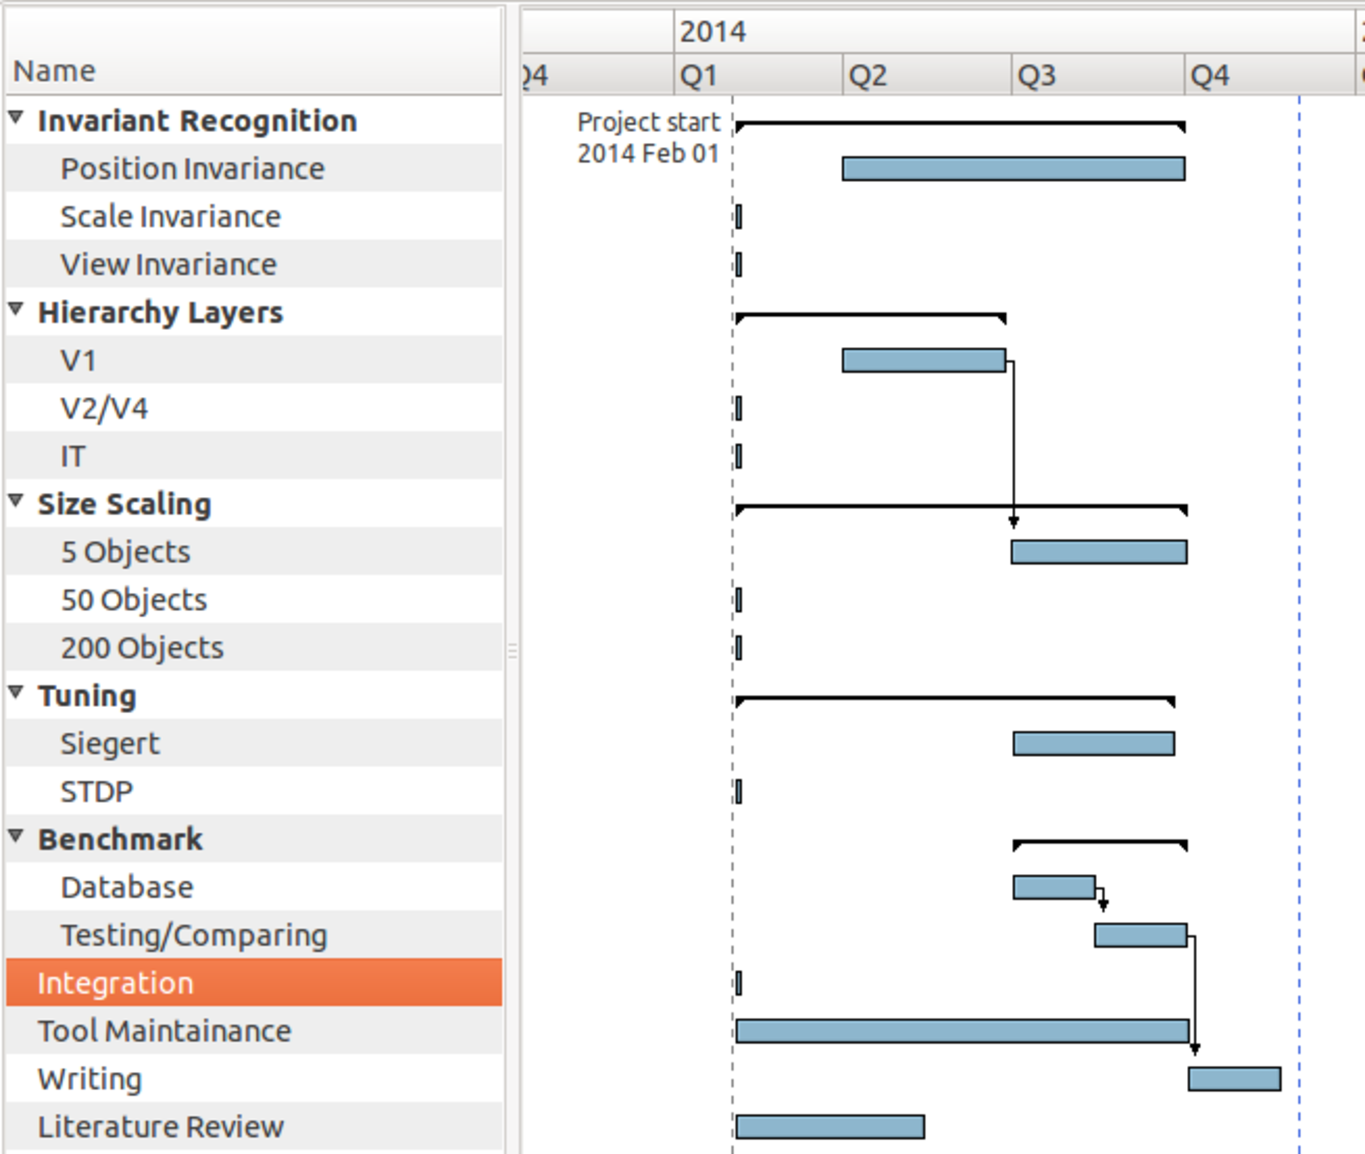
\includegraphics[width=0.8\textwidth]{pics/gantt.pdf}
	\caption{Gantt chart of the work flow for the first milestone.
	The main research works are listed on the left.
%	Different from the example, in the following work, not only achieving a milestone but also any increase in any dimension will result in tuning and benchmark testing.
	}
	\label{Fig:gantt}
\end{figure}
\subsection{Invariant Object Recognition}
As stated previously the brain recognises huge number of objects rapidly with ease even in noisy natural scenes. We will explore the invariant object recognition in three features: position, scale and viewing angle.
%While the major stumbling crux of the computer object recognition systems lies in the invariance problem.
%To explore the invariant object recognition of the brain in a biologically plausible way is the right place to solve the computational difficulty.
\subsubsection{Position Invariance}
Position invariance in the lower level of V1-liked neurons has been achieved in the preliminary work by convolving receptive fields with Gabor kernels.
The following work in accordance with Figure~\ref{Fig:3Dplan} will focus on expanding the position invariance to higher hierarchical levels of the ventral stream.
\subsubsection{Scale Invariance}
Similar to orientation detection, V1 provides overcomplete population re-representations of visual image on the features of scale, frequency and orientation.
It forms the basis of scale invariant object recognitions.
Likewise, integrating the features into the higher abstraction of layered network to recognise more complex figures will require a tense work on tuning.
\subsubsection{View Invariance}
A difficult specificity-invariance trade-off occurs in view invariant recognition tasks, since the recogniser should be able to discriminate different objects while at the same time also tolerating to viewing angle transformations.
Learning will play a very important role in this work, where objects observed with multiple view points can be recognised even if only single view point is presented during training.
\subsection{Modelling the Ventral Visual Pathway}
As the visual information propagates through the ventral stream (via visual area V1, V2/V4 and IT), neurons become selective for increasingly complex features. 
Along with this growing complexity of the preferred stimulus, neurons become more and more tolerant to the position and scale of the stimulus within their receptive fields.
Inspired from the functional behaviour of the biological data (many have been mentioned in Section~\ref{sec:bio}), this work will mimic the neural activity of each hierarchy layer by LIF neurons.
 
%To satisfy the functional discoveries, this work will employ learning and compare with biological data.
%This work will ask for a close collaboration with neuroscience to gather biological data for both training and testing.
\subsection{Size Scaling}
The milestones set for the dimension of number of classes/objects is in accordance with experimental data from the study of neuroscience.
In work by~\cite{hegde2004temporal}, the classical receptive field of the V2 cell consists of 48 grating stimuli and 80 contour stimuli; while Zoccolan et al.~\cite{zoccolan2007trade} tested and recorded the activity of the IT neurons of monkeys with 213 grayscale pictures of isolated real-world objects.

Thanks to the massively-parallel neural simulations possible in the SpiNNaker system, implementing real-time invariant object recognition becomes possible.
However, it also requires the supporting software development to support larger neural networks than currently possible.  
\subsection{Integration}
To reach the milestone of building an object recognition system with position, scale and view invariance, integration of these separate models will be a challenge.
It not only requires placing the models physically together but also merging their functions.
As illustrated in Section~\ref{sec:orIT}, single neurons are tuned to different features and object identities.
This work requires further investigation into population coding and learning. 
\subsection{Tuning}
Tuning is the key to make the object recognition system a success.
In preliminary work, Siegert transformation functions are used to adjust perceptral weights for spiking LIF neurons.
This is a strong indicator of the feasibility of the work.
However, learning algorithms such as STDP in spiking neural networks are must be employed to make the system more biologically plausible.
It is hoped that, this work will provoke further study of learning algorithms on SpiNNaker.
\subsection{Benchmarking Performance}
The performance of the real-time recognition system will be evaluated of each milestone to validate the success of the models.
The neural activities and recognition rate will be compared with biological data which will act as a benchmark.
\subsubsection{Building a Dataset}
Building a well-labelled retinal output dataset is essential in spike-based object recognition study.
Unified benchmarks with AER format will be ideal for SNN study, because of its non-frame, event-based fashion.
These benchmark datasets will also make it possible for other researchers to test their SNN model without a silicon retina present.
It is hoped that this would boost communication, comparison and collaboration within the community.
This work also requires lively discussion and cooperation with neuroscientists, where data can be derived and tested.
\subsubsection{Testing/Comparing}
The testing and comparing on the dataset will verify the reliability of the models.
The neural responses of single or populated neurons to the same dataset will be analysed in firing rate and response time.
By comparing with the biological data, the model can be rectified and improved.
The more data it compares with, the closer it could untangle the object representation. 


%\subsection{Optional: Action Recognition}
%vision attention.
%short-term memory.
%\subsection{Optional: Sensor Fusion with Auditory Processing}
%platform.
%applications as lip-reading and speaker identification.


\chapter{Conclusion}
\label{cha:con}
%Motivation
To explore how brain may recognise objects in its general, accurate and energy-efficient manner, this paper proposes the use of a neuromorphic hardware system which includes a DVS retina connected to SpiNNaker, a real-time SNN simulator.
%Problem
Building a recognition system based on this bespoke hardware for dynamic hand postures is a first step in the study of visual pathway of the brain.
%Methods
Inspired by the structures of the primary visual cortex, convolutional neural networks are modelled using both linear perceptrons and LIF neurons.
%Results
The larger network of 74,210 neurons and 15,216,512 synapses runs smoothly in real-time on SpiNNaker using 290 cores within a 48-node board.
The smaller network using 1/10 of the resources is able to recognise the postures in real-time with an accuracy about 86.4\% in average, which is 
only 6.6\% lower than the former but with a better cost/performance ratio.
%In this paper, we implement a dynamic hand posture recognition system running completely on a hardware neuromorphic platform.
%The SNN based classifier is able to recognise moving hand postures instead of static digit or face recognition proposed before.
%The network model is translated from linear perceptrons to LIF spiking neurons with a 10\% drop of accuracy in 30~ms windowing;
%while the performance reaches and even exceeds the perceptrons version when the window length is set to 300~ms.
%Various network sizes are configured to explore the cost and performance trade-off.
%In the tests of linear perceptrons the recognition rate of the smaller network is \% lower for the template matching model and \% lower for the trained MLP model.
%For the SNN based real-time experiments, both the larger network with $74,320$ LIF neurons and $15,216,512$ synapses, and the smaller network with 1/10 of the neurons and 1/50 of the synapses run smoothly on SpiNNaker.
%The gap of recognition rate narrows when the spiking rate is sampled into wider frame of 300~ms.
%The recognition rates of both linear perceptrons (\%) and spiking neurons (\%) with 32 $\times$ 32 input resolution are adequate for the recognition of the moving hand postures.
%This work is a good attempt to start exploring the visual process of the brain.

%Later, we will look more into the overall network latency, which could be due to the system latency and the performance of the rate coding.  
The future work on this topic will include further collaboration with biologists and neuroscientists working on vision systems, especially concentrating on the orientation detection region of the brain.
To equip the system with tracking is another importance direction for future development where the recognition performance can be increased by exploiting short-term memory of a gesture's route.
Using the approch of HMMs~\cite{elmezain2009hidden} and applying to spiking neural networks is an idea we wish to explore as part of this promising work.
%Using the idea of HMMs~\cite{elmezain2009hidden} to spiking neural networks may be a good approach. 


\bibliography{refs}    % this causes the references to be listed

%\bibliographystyle{alpha}
\bibliographystyle{ieeetr}
%% the bibliography style determines the format  in which both citations and references are printed,
%% other possible values are plain and abbrv
%%
%% If you want more control of the format of your citations you might want to take a look at
%% natbib.sty, which should be part of any standard LaTeX installation
%%
%% University regulations simply require that your citation style be consistent, so see what style
%% your supervisor recommends.

\end{document}
